\section{Resultados}
%%%%%%%%%%%%%%%%%%%%%

Los resultados deben referirse a lo que se obtiene siguiendo la metodolog�a:
ni se juzgan, ni se dan opiniones, aunque s� se pueden anotar condiciones
particulares.

%Tabla
\begin{table}[tbh]
    \caption{\label{tab:tiempos}Tiempo empleado en cada paso.}
    \begin{centering}
        \begin{tabular}{|c|c|c|c|}
            \hline
            Paso      & Tiempo    & Paso       & Tiempo                                \\
            \hline
            \csvreader[late after line= \\]{./files/data.csv}{}% use head of csv as column names
            {\csvcoli & \csvcolii & \csvcoliii & \csvcoliv}% specify your columns here
            \hline
        \end{tabular}
    \end{centering}
\end{table}

Por ejemplo, siguiendo la metodolog�a del apartado \ref{sub:metodo},
se ha llegado al resultado de la figura \ref{fig:resultado}. El tiempo
empleado en escribir la plantilla se muestra en la tabla \ref{tab:tiempos}
seg�n los pasos indicados en la metodolog�a
%Nota al pie:
\footnote{El tiempo invertido en la primera escritura (paso 2) es s�lo estimativo,
    ya que se desarroll� paralelamente a otras actividades a lo largo
    de varios d�as.
}.

%Figura
\begin{figure}[tbh]
    \begin{centering}
        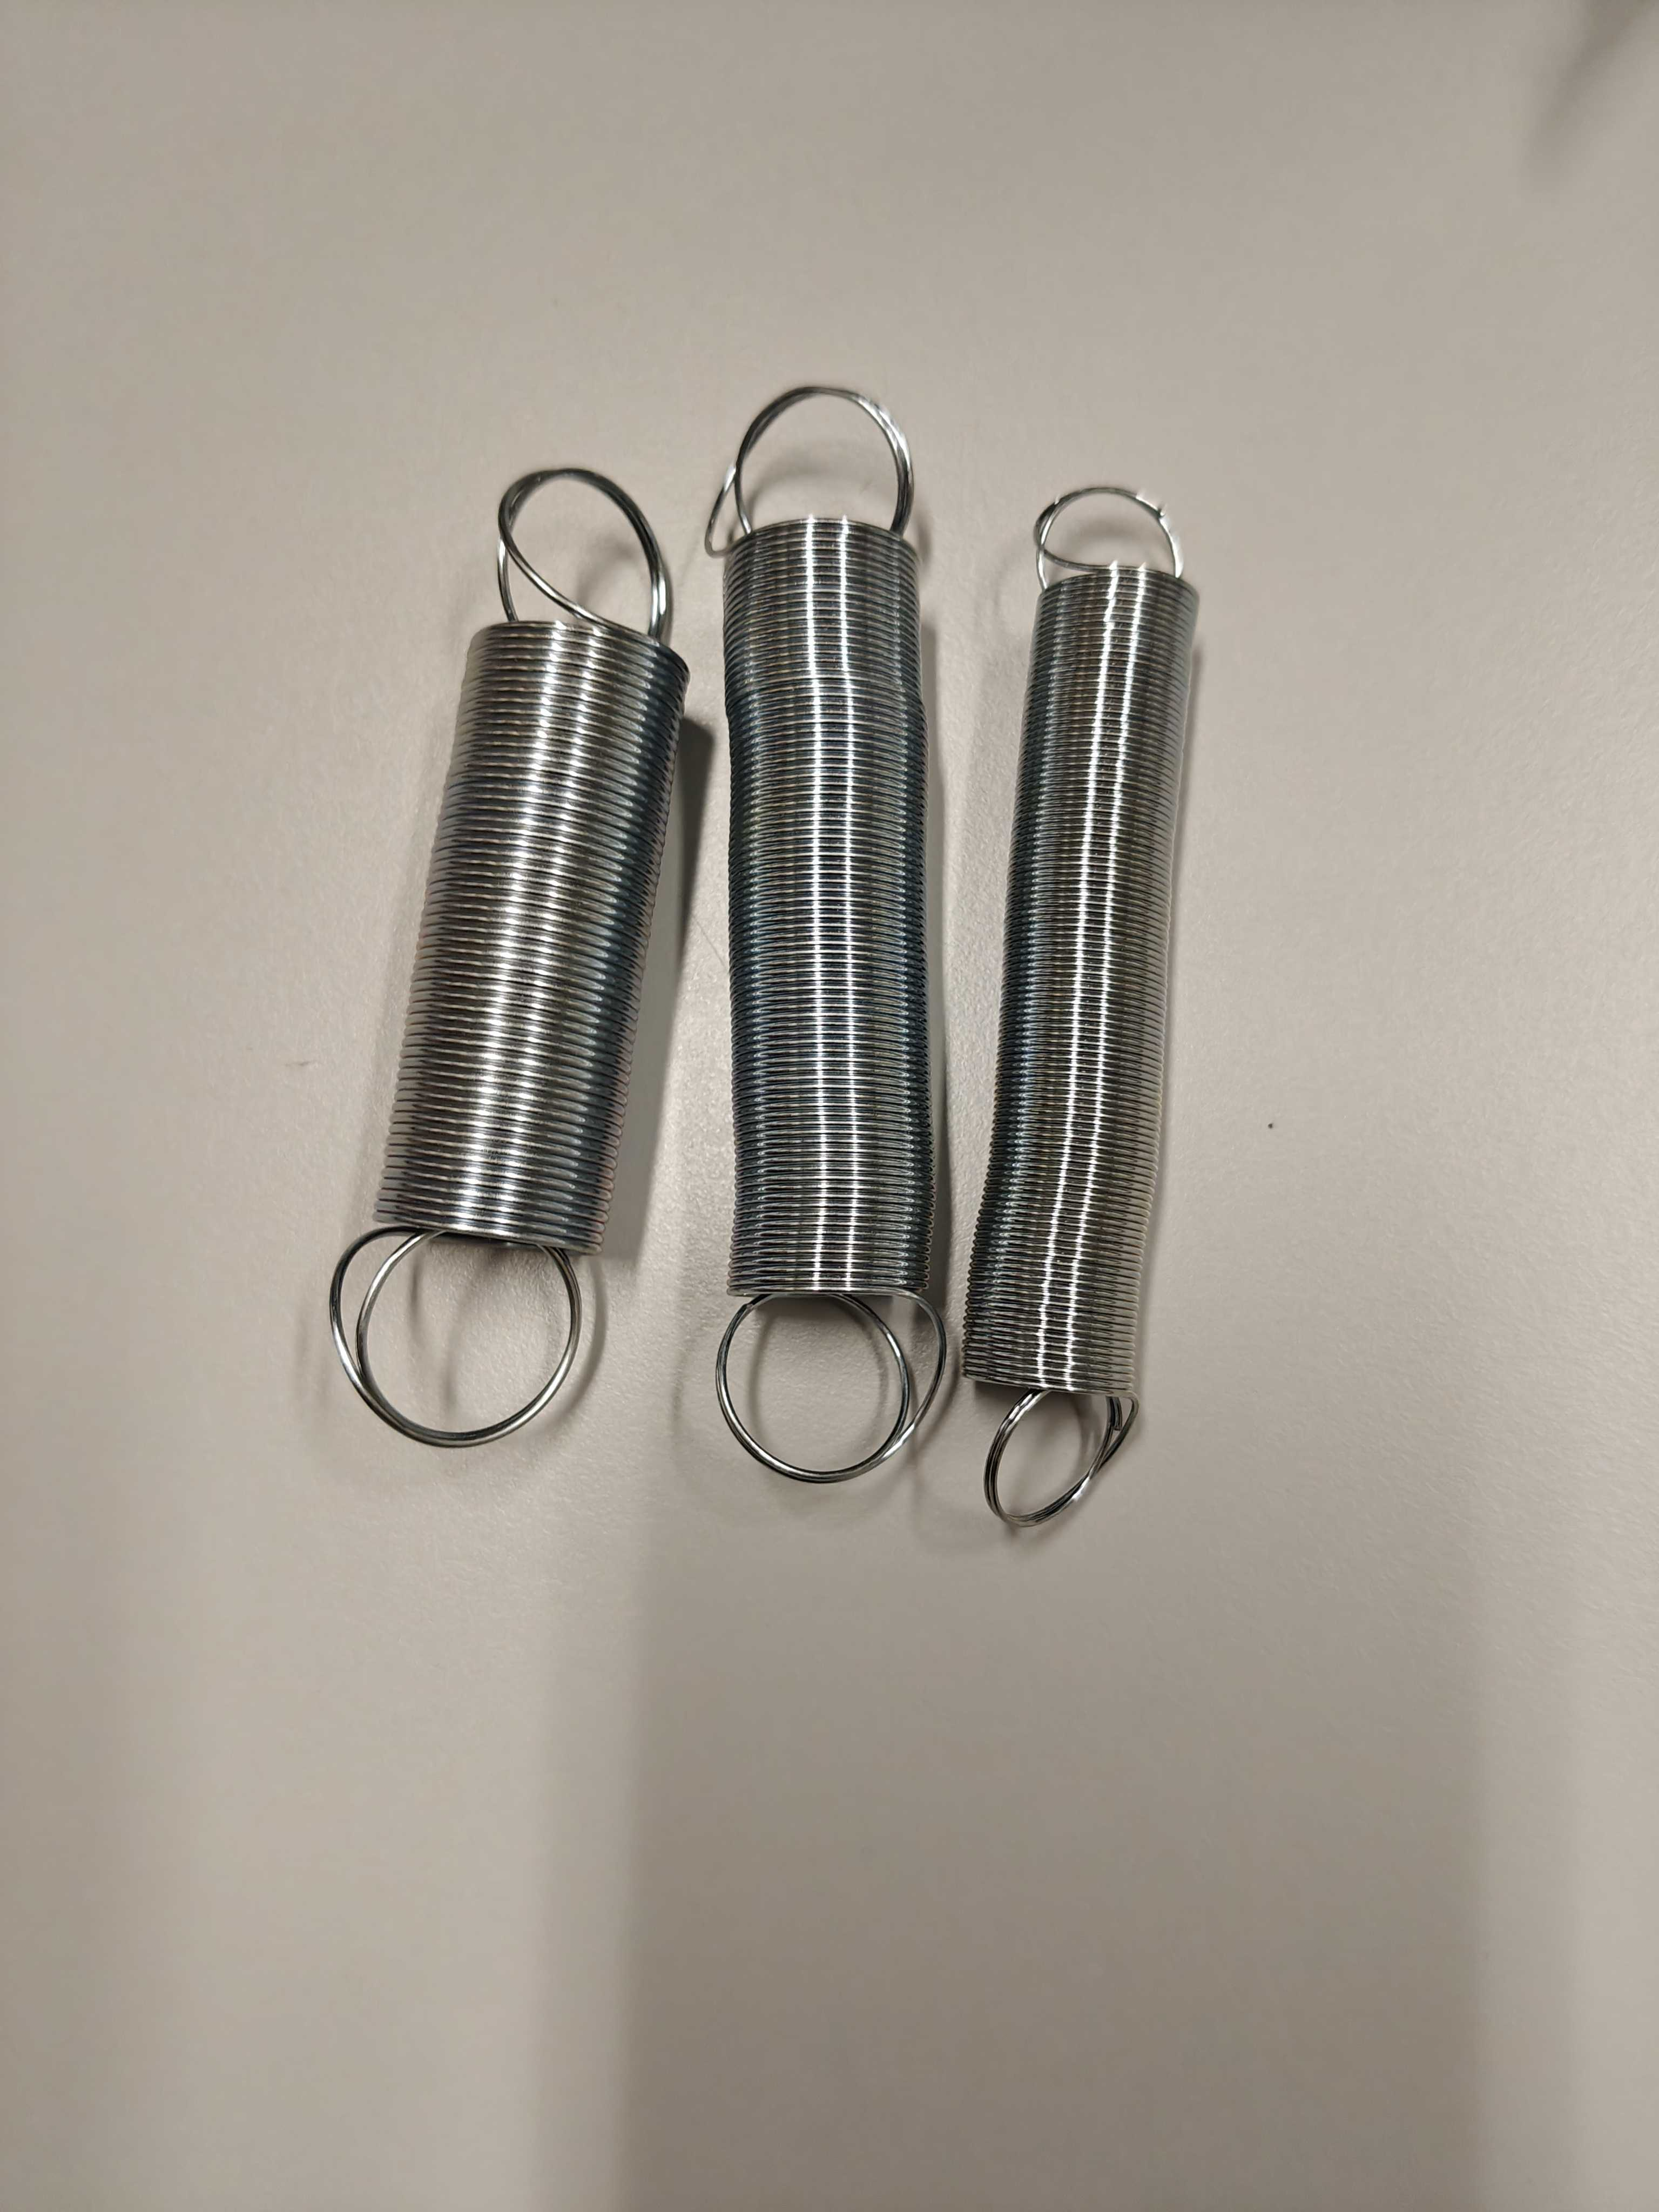
\includegraphics[width=0.8\columnwidth]{files/muelles}
    \end{centering}
    \caption{\label{fig:resultado}Miniatura de la primera p�gina de la plantilla
    de memoria.}
\end{figure}

